\documentclass[11pt,letterpaper]{article}
\usepackage[T1]{fontenc}
\usepackage[utf8]{inputenc}
\usepackage{lmodern,amsmath,amssymb,amsthm,mathtools}
\usepackage[margin=1in]{geometry}
\usepackage{microtype,booktabs,array,longtable,enumitem,xcolor}
\usepackage{tikz}
\usetikzlibrary{arrows.meta,positioning}
\usepackage{fancyhdr}
\usepackage{listings}
\usepackage[hidelinks,breaklinks]{hyperref}
\usepackage[nameinlink,noabbrev]{cleveref}
\hypersetup{pdftitle={Twist-Compressed Khovanov Recognition},pdfauthor={Research report prepared for the ProveIt project},pdfsubject={Explicit complexity bounds and an opt-in exact unknot-recognition backend}}
\setlength{\headheight}{14pt}
\pagestyle{fancy}
\fancyhf{}
\fancyhead[L]{\small ProveIt / Unknot Recognition}
\fancyhead[R]{\small Twist compression and certified cost bounds}
\fancyfoot[C]{\thepage}
\setlength{\parskip}{4pt}
\setlength{\parindent}{1.2em}
\setlist{nosep,leftmargin=1.8em}
\newtheorem{theorem}{Theorem}[section]
\newtheorem{lemma}[theorem]{Lemma}
\newtheorem{proposition}[theorem]{Proposition}
\newtheorem{corollary}[theorem]{Corollary}
\theoremstyle{definition}
\newtheorem{definition}[theorem]{Definition}
\newtheorem{remark}[theorem]{Remark}
\newtheorem{question}[theorem]{Research question}
\newcommand{\F}{\mathbb F_2}
\newcommand{\Z}{\mathbb Z}
\newcommand{\Kh}{\operatorname{Kh}}
\newcommand{\rKh}{\widetilde{\operatorname{Kh}}}
\newcommand{\tr}{\operatorname{tr}}
\newcommand{\TL}{\operatorname{TL}}
\newcommand{\poly}{\operatorname{poly}}
\newcommand{\supp}{\operatorname{supp}}
\newcommand{\rank}{\operatorname{rank}}
\newcommand{\N}{\mathcal N}
\newcommand{\U}{\mathcal U}
\newcommand{\eps}{\varepsilon}
\newcommand{\code}[1]{\texttt{\detokenize{#1}}}
\lstset{basicstyle=\small\ttfamily,breaklines=true,columns=fullflexible,keepspaces=true,frame=single,rulecolor=\color{black!25},xleftmargin=0.5em,xrightmargin=0.5em}
\begin{document}
\begin{titlepage}
\thispagestyle{empty}
\vspace*{0.25in}
\noindent{\large\scshape ProveIt research report}\par
\vspace{0.35in}
\noindent{\Huge\bfseries Twist-Compressed\\[5pt] Khovanov Recognition}\par
\vspace{0.2in}
\noindent{\Large Explicit complexity bounds, exact cost certificates,\\and a tested route toward quasi-polynomial time}\par
\vspace{0.25in}
\noindent Prepared for Vladimir Reshetnikov's ProveIt project\par
\noindent 7 October 2026\par
\vspace{0.2in}\hrule\vspace{0.2in}
\begin{abstract}
We develop an opt-in exact unknot-recognition backend for closures of braids
\(\beta=\sigma_{i_1}^{e_1}\cdots\sigma_{i_t}^{e_t}\), where
\(m_j=|e_j|\) and \(n=\sum_jm_j\). Standard local two-strand Khovanov simplifications replace each crossing cube by a complex with \(m_j+1\) terms. We derive an exact support polynomial for the resulting reduced chain dimension,
\[
 \N=\sum_{S\subseteq[t]}2^{c(S)-1}\prod_{j\in S}m_j,
\]
and prove the sharper first-use bound
\[
 \N\leq \U:=\prod_{i=1}^{b-1}\frac{3+\prod_{j:i_j=i}(1+2m_j)}2.
\]
For a one-component closure every Artin generator occurs, so
\(\U\leq\prod_j(1+2m_j)\leq(1+2n/t)^t\).
Exact linear algebra therefore gives a complete recognition algorithm in
\(\poly(n)\,2^{O(t\log(2+n/t))}\) bit operations. In particular, the algorithm is polynomial for bounded \(t\) and quasi-polynomial when \(t=O(\log n)\).

We also give a Temperley--Lieb transfer algorithm that computes the exact chain-size and degree-profile certificates without building the chain complex, a sharp contextual formula for the savings from coalescing twist blocks, and an explicit bounded-width family exhibiting exponential chain multiplicity. The implementation passes 62 unit tests and 900 comparisons against an independently assembled crossing cube, including differential-square and degree-count checks. Controlled same-code ablations and raw measurements are included.

The unrestricted quasi-polynomial target is not established. Local twist normal forms are existing mathematics, not a novelty claim. The additional contributions are the explicit counting and complexity analysis, the first-use refinement, the cost-certificate algorithms, and the accompanying implementation. A final section formulates precise progress-state budgets for the separate hierarchy route.
\end{abstract}
\vfill
\noindent\small\textbf{Scope.} Explicit braid words; reduced Khovanov homology over \(\F\); quantum grading forgotten. The package is not a drop-in replacement for the current optimized scanner. Upstream cross-validation is supplied as an integration gate but was not executed in this session.
\end{titlepage}
\setcounter{tocdepth}{1}
\tableofcontents
\newpage

\section{Research position and repository audit}
\subsection{What the present work changes}
The performance objective is not simply to make the next crossing cheaper.
It is to avoid constructing exponentially many copies of the same local information. A twist block is a particularly clean place to do this: its local homotopy type has a small explicit representative, and the geometric part of a global state depends only on whether that block contributes the identity smoothing or the turnback smoothing. The internal position along its local complex affects the degree and differential, but not the underlying matching.

This report separates three quantities that must not be conflated:
\begin{equation}\label{eq:threecounts}
\begin{aligned}
 G&=\text{number of geometric matching types},\\
 M&=\text{number of copies of those types in a chain complex},\\
 B&=\text{bits needed to record their dimensions}.
\end{aligned}
\end{equation}
The first may be bounded while the second is exponential. The third may remain polynomial even when the second is exponential. The backend improves the second quantity on twist-structured inputs; the preflight algorithms exploit the third quantity on a wider collection of inputs.

The proposed integration target is a new directory, for example
\path{Topology/UnknotRecognition/research/twist_compression/}.
No existing default is changed by this package. In particular, the performance measurements below are neither a replacement for nor a claimed speedup over the repository's optimized \code{fastunknot.scan}.

\subsection{The code that was reviewed}
The repository currently documents an exact but worst-case exponential pipeline, including Reidemeister reductions, descending-diagram recognition, visible connected-sum factorization, modular Alexander and Jones obstructions, and a reduced Khovanov endpoint \cite{repo}. The implementation in \code{recognize.py} is slightly more specific than the introductory README: exact Alexander computation is normally skipped when the modular Alexander stage has already run, and Reidemeister III search is delayed until the filters have failed. These are existing improvements and are not credited to the present report.

The reviewed scanner already uses several techniques that a new proposal should not rediscover: bit-packed morphisms, local gluing plans, unit cancellation, fill-sensitive pivot selection, and alternative scan orders. The root README explicitly withholds a quasi-polynomial guarantee. We retain that distinction. The exact files and content identifiers reviewed are listed in \cref{app:provenance}; the complete checkout and its unit suites were not run here.

A useful consequence of this audit is architectural. A new algebraic backend belongs after inexpensive exact obstructions, not before them. Moreover, the current \code{Diagram} stores a planar diagram, not the original braid word. A twist-block backend needs retained braid provenance or a separately verified conversion. It must not assume that a braid for the original input also represents a factor produced by later planar-diagram cuts.

\subsection{Primary literature and limits of novelty}
The local input is established: Bar-Natan's tangle formalism and local cancellation machinery \cite{bn05,bn07}, with an explicit integer-twist normal form in Thompson's Proposition 4.1 \cite{thompson}. The unknot decision criterion comes from Kronheimer--Mrowka \cite{km}. We use these theorems; we do not claim to reprove or originate them.

A particularly relevant recent result is Kelom\"aki--Sch\"utz \cite{ks26}: their Theorem 1.3 gives polynomial-time Khovanov computation for all three-strand braids, whereas Theorem 1.2 proves exponential behavior for basis-expanding scanning on certain three-strand families. Thus bounded strand number is not a valid justification for bounding the size of an explicit reduced complex. Our bounded-run theorem applies to arbitrary strand counts, but is not an improvement over their specialized theorem on all three-strand inputs.

For the hierarchy route, Lackenby's July 2026 preprint \cite{lackenby26}, Section 9, distinguishes a bound on iterations from a fully costed implementation. Proposition 9.1 gives \(L(g+1)^L\) iterations in terms of hierarchy length and pattern-complexity bounds. The April 2021 Princeton announcement \cite{lackenby21} states \(2^{O((\log n)^3)}\), so even the phrase ``quasi-polynomial'' does not specify the exponent of the logarithm. Here the restricted-family target is the stronger \(2^{O((\log n)^2)}=n^{O(\log n)}\).

\begin{center}
\small
\begin{tabular}{p{0.46\linewidth}p{0.45\linewidth}}
\toprule
Statement & Status in this report\\
\midrule
Local two-strand normal form and unknot detection by Khovanov rank & Existing theorems, explicitly attributed.\\
Support polynomial, first-use bound, trace certificates, coalescence gap & Derived and proved below.\\
Complete quasi-polynomial recognition for \(t=O(\log n)\) & A proved restricted-input consequence.\\
Python backend and exact preflight routines & Implemented and independently tested.\\
Faster end-to-end recognition than the current ProveIt scanner & Not established; upstream timing and integration remain to be run.\\
Quasi-polynomial recognition on every input diagram & Not established.\\
\bottomrule
\end{tabular}
\end{center}
Priority in the published literature for each elementary counting refinement has not been exhaustively established. The proofs and artifacts, rather than a claim of unprecedented discovery, are the basis for integrating this work.

\section{Input model and the local complex}\label{sec:local}
\subsection{Signed runs and the size parameter}
Let \(b\geq1\) and let \(\beta\) be a braid on \(b\) strands, written as
\begin{equation}\label{eq:braid}
 \beta=\sigma_{i_1}^{e_1}\cdots\sigma_{i_t}^{e_t},
 \qquad 1\leq i_j<b,\quad e_j\in\Z\setminus\{0\}.
\end{equation}
Write \(m_j=|e_j|\), \(\eps_j=\operatorname{sign}(e_j)\), and
\(n=\sum_jm_j\). A block is homogeneous in sign. Maximal equal signed letters in an explicit word give one canonical initial grouping. Our theorems also allow nonmaximal grouping; that is useful for controlled ablation and for the coalescence identity in \cref{sec:merge}.

The parameter \(t\) is a property of the supplied presentation. It is not braid index, minimal syllable length under all braid relations, or the diagrammatic twist number of a general planar diagram. No efficient procedure producing \(t=O(\log n)\) for every knot is asserted.

The asymptotic variable \(n\) is the expanded number of crossings. A JSON run exponent can be binary encoded; an exponent of magnitude \(2^q\) still contributes \(2^q\) to \(n\), not \(q\). The recognition theorem is not a polynomial or quasi-polynomial bound in binary-encoded exponent length. In contrast, the scalar preflight trace can sometimes process such exponents directly, because it never expands the local degree interval.

\subsection{Smoothings, grading, and the marked circle}
Let \(I\) denote two vertical arcs and \(E\) the turnback with a top cup and bottom cap, with all other braid strands vertical. The mark lies on a closing arc of strand zero, outside every twist box.

\begin{figure}[ht]
\centering
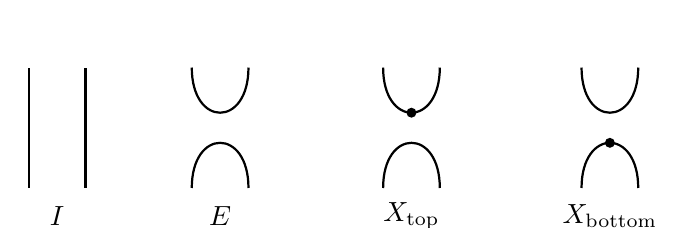
\begin{tikzpicture}[scale=0.9,line width=0.8pt]
 \draw (0,0)--(0,1.7);\draw (0.8,0)--(0.8,1.7);
 \node at (0.4,-0.4){\(I\)};
 \draw (2.3,1.7) .. controls (2.3,0.85) and (3.1,0.85) .. (3.1,1.7);
 \draw (2.3,0) .. controls (2.3,0.85) and (3.1,0.85) .. (3.1,0);
 \node at (2.7,-0.4){\(E\)};
 \draw (5.0,1.7) .. controls (5.0,0.85) and (5.8,0.85) .. (5.8,1.7);
 \draw (5.0,0) .. controls (5.0,0.85) and (5.8,0.85) .. (5.8,0);
 \fill (5.4,1.0625) circle (2pt);
 \node at (5.4,-0.4){\(X_{\rm top}\)};
 \draw (7.8,1.7) .. controls (7.8,0.85) and (8.6,0.85) .. (8.6,1.7);
 \draw (7.8,0) .. controls (7.8,0.85) and (8.6,0.85) .. (8.6,0);
 \fill (8.2,0.6375) circle (2pt);
 \node at (8.2,-0.4){\(X_{\rm bottom}\)};
\end{tikzpicture}
\caption{The two underlying smoothings and the two dot endomorphisms of \(E\). Dots indicate multiplication by \(X\) on the indicated sheet, not extra generators of a geometric state.}
\label{fig:smoothings}
\end{figure}

We use the Frobenius algebra
\[
 A=\F[X]/(X^2),\qquad
 \Delta(1)=1\otimes X+X\otimes1,\qquad
 \Delta(X)=X\otimes X.
\]
A smoothing with \(c\) circles has reduced space
\(XA\otimes A^{\otimes(c-1)}\), of dimension \(2^{c-1}\).
The marked circle is constrained to the label \(X\). On unmarked circles a bit records whether the label is \(1\) or \(X\).

Our homological grading is normalized so that a positive crossing has
\(I\to E\) in degrees \(0,1\), and a negative crossing has
\(E\to I\) in degrees \(-1,0\). Quantum grading is deliberately forgotten throughout the implementation. This does not change total reduced rank or the normalized homological degree counts.

\begin{proposition}[Standard twist normal form]\label{prop:normal}
In the dotted Khovanov category over \(\F\), after forgetting quantum grading, a positive \(m\)-crossing two-strand twist has a representative
\[
 I\xrightarrow{s} E\xrightarrow{D}E\xrightarrow{D}\cdots\xrightarrow{D}E,
 \qquad D=X_{\rm top}+X_{\rm bottom},
\]
with one term in each degree \(0,1,\ldots,m\). A negative twist has the dual representative, one term in degrees \(-m,\ldots,-1,0\), with \(I\) at degree zero, a final saddle into \(I\), and the same internal dot sum.
\end{proposition}
\begin{proof}
This is the mod-two, quantum-ungraded specialization of the integer-twist normal form in \cite[Proposition 4.1]{thompson}, after choosing the braid orientation above. Its local proof tensors a twist complex with one crossing, deloops every \(E\circ E=E\sqcup\bigcirc\), and cancels the resulting identity entries. Delooping replaces a circle by two summands; categorical elimination replaces the remaining block by the Schur complement
\(\epsilon-\gamma\phi^{-1}\delta\) \cite[Lemmas 4.1--4.2]{bn07}.
The surviving internal maps alternate dot difference and dot sum over the integers; these agree over \(\F\). Mirroring dualizes the complex and reverses homological degrees. All operations are relative to the boundary, so the replacement can be made inside any larger planar composition.
\end{proof}

Two checks illuminate the formula but do not replace the homotopy-equivalence theorem. First,
\(D^2=X_{\rm top}^2+2X_{\rm top}X_{\rm bottom}+X_{\rm bottom}^2=0\).
Second, the two dotted compositions next to an endpoint saddle agree by dot sliding and therefore cancel over \(\F\). Different boxes commute, and their two orders of application cancel in the total differential.

After closure the top and bottom arcs of an \(E\) term may belong to the same circle. In that case the two dots cancel. A dot on the marked circle is zero because \(X^2=0\). Both phenomena must be handled explicitly: a symbolic ``two dots'' record is not automatically a nonzero matrix column.

\section{Exact chain size and a sharper first-use bound}\label{sec:count}
\subsection{The support polynomial}
A macro state is a tuple
\(k=(k_1,\ldots,k_t)\) with \(0\leq k_j\leq m_j\).
Its homological degree is \(h(k)=\sum_j\eps_jk_j\).
The \(j\)-th box is \(I\) when \(k_j=0\), and \(E\) otherwise. Consequently its geometry depends only on
\(S(k)=\{j:k_j>0\}\), not on the nonzero values themselves.
Let \(c(S)\) be the number of circles obtained by composing those smoothings and closing the braid.

\begin{theorem}[Exact support polynomial]\label{thm:polynomial}
The total dimension of the reduced macro chain complex is exactly
\begin{equation}\label{eq:exactN}
 \N(\beta)=\sum_{S\subseteq[t]}2^{c(S)-1}\prod_{j\in S}m_j.
\end{equation}
Its degree-dimension polynomial is
\begin{equation}\label{eq:profile}
 P_\beta(z)=\sum_h\dim C^h\,z^h
 =\sum_{S\subseteq[t]}2^{c(S)-1}
        \prod_{j\in S}(z^{\eps_j}+\cdots+z^{m_j\eps_j}).
\end{equation}
In particular, \(P_\beta(1)=\N(\beta)\).
\end{theorem}
\begin{proof}
For each fixed support \(S\), there are exactly \(\prod_{j\in S}m_j\) choices of nonzero local indices. Each choice contributes the same reduced space of dimension \(2^{c(S)-1}\). Summing over supports proves \cref{eq:exactN}. Keeping the homological degree of each choice gives \cref{eq:profile}. No cancellation in the differential has yet been used, so these are exact chain dimensions, not estimates of Betti numbers.
\end{proof}

A first bound, obtained by replacing each \(I\) by \(E\) one at a time, is
\(c(S)\leq b+|S|\), hence
\(\N\leq2^{b-1}\prod_j(1+2m_j)\).
The following refinement is substantially better and costs almost nothing to evaluate.

\begin{lemma}[First use of a generator]\label{lem:first}
Let
\(d(S)=|\{i_j:j\in S\}|\) be the number of distinct Artin generator indices represented in \(S\). Then
\begin{equation}\label{eq:first}
 c(S)\leq b+|S|-2d(S).
\end{equation}
Moreover, \(b+|S|-2d(S)-c(S)\) is an even nonnegative integer.
\end{lemma}
\begin{proof}
Begin with every box equal to \(I\), giving \(b\) circles. Activate the \(E\) boxes of \(S\) in the order in which they occur in the word. Each activation is a saddle, so it changes the number of circles by either \(+1\) or \(-1\).

Consider the first activation with generator index \(i\). Before it, no active turnback crosses the cut between positions \(i\) and \(i+1\). Every existing connection, including closure arcs, stays entirely on one side of that cut. The two local vertical arcs therefore belong to different circles. The activation merges them, changing the circle count by \(-1\), rather than the \(+1\) allowed in the crude bound.

There are \(d(S)\) such first activations. Every other activation changes the count by at most \(+1\). Starting from \(b\), this yields
\(b-d(S)+(|S|-d(S))\). Replacing any of the remaining \(+1\)'s by \(-1\) decreases the result by two, proving the parity assertion as well.
\end{proof}

\begin{theorem}[Generator-sensitive product bound]\label{thm:generator}
For \(1\leq i<b\), set
\[
 Q_i=\prod_{j:i_j=i}(1+2m_j),
\]
with empty product one. Then
\begin{equation}\label{eq:U}
 \N(\beta)\leq\U(\beta):=\prod_{i=1}^{b-1}\frac{3+Q_i}{2}.
\end{equation}
All factors on the right are integers. If the closure has one component and \(t>0\), then
\begin{equation}\label{eq:AMGM}
 \N(\beta)\leq\U(\beta)
 \leq\prod_{j=1}^t(1+2m_j)
 \leq\left(1+\frac{2n}{t}\right)^t.
\end{equation}
\end{theorem}
\begin{proof}
Insert \cref{eq:first} into \cref{eq:exactN}. The contribution of \(S\) is at most
\(2^{b-1}4^{-d(S)}\prod_{j\in S}(2m_j)\).
Partition the choices in \(S\) according to their generator index. Within the group for index \(i\), the empty choice contributes one. The nonempty choices contribute
\(\frac14(Q_i-1)\). Thus
\[
 \N\leq2^{b-1}\prod_{i=1}^{b-1}\left(1+\frac{Q_i-1}{4}\right)
      =\prod_{i=1}^{b-1}\frac{Q_i+3}{2}.
\]
Each \(Q_i\) is odd, so the factors are integral.

If a generator index \(i\) never occurs in a braid word, its permutation preserves the nonempty sets of positions to the left and right of that cut. The closure then has at least two components. Therefore, in a one-component closure every index occurs, so \(Q_i\geq3\) and
\((Q_i+3)/2\leq Q_i\). Multiplying gives the middle inequality. The last inequality is arithmetic--geometric mean applied to the positive numbers \(1+2m_j\), whose sum is \(t+2n\).
\end{proof}

\begin{remark}[Sharpness and what is being bounded]
For two strands all active boxes use one generator, and after the first activation every further activation creates a circle. Thus \cref{eq:U} is an equality:
\(\N=(3+\prod_j(1+2m_j))/2\).
It is also an equality when every generator occurs in at most one box. In particular, a single twist has \(\N=m+2\), not \(2^{m}\).
These are statements about the selected complex, not topological invariants. Its dimension can change drastically under a braid relation or a different grouping of an identical word.
\end{remark}

For additional geometric information define the nonnegative integer
\[
 \gamma(S)=\frac{b+|S|-2d(S)-c(S)}2.
\]
The exact support summand is the first-use upper summand multiplied by \(4^{-\gamma(S)}\). This identifies precisely the loss in the product bound. We use \(\gamma\) only as this combinatorially defined defect; no identification with a genus of an unspecified embedded surface is needed.

\section{Cost certification without expanding the complex}\label{sec:trace}
\subsection{A scalar Temperley--Lieb trace}
Work in the diagrammatic Temperley--Lieb algebra \(\TL_b(2)\) over \(\Z\). A closed internal circle has value \(2\), the identity matching is \(I\), and \(E_i\) joins neighboring top endpoints and neighboring bottom endpoints. Let \(\tr_2\) be the ordinary closure trace: a matching closing to \(c\) circles has trace \(2^c\).

This is a chain-dimension calculation over the integers. It is not a Jones-polynomial evaluation over \(\F\), and is not a knot invariant. The differential has deliberately been discarded.

\begin{theorem}[Exact trace certificates]\label{thm:trace}
The support polynomial and degree profile admit the expressions
\begin{align}
 \N(\beta)&=\frac12\tr_2\prod_{j=1}^t(I+m_jE_{i_j}),\label{eq:traceN}\\
 P_\beta(z)&=\frac12\tr_2\prod_{j=1}^t
       \left(I+(z^{\eps_j}+\cdots+z^{m_j\eps_j})E_{i_j}\right).
       \label{eq:traceP}
\end{align}
The scalar expression can be evaluated using at most \(C_b=\frac1{b+1}\binom{2b}{b}\) matching states per step, without enumerating the \(\prod_j(m_j+1)\) macro states.
\end{theorem}
\begin{proof}
Expanding either product chooses \(I\) or \(E\) in each box. Internal loops created during composition contribute the same factors of two as the circles counted at final closure. For support \(S\), the full trace is therefore \(2^{c(S)}\). The mark removes one factor of two, giving the prefactor \(1/2\) and \cref{eq:exactN,eq:profile}. The division is integral since there is at least one closing circle.

A \(b\)-strand matching is a noncrossing pairing of \(2b\) boundary endpoints in their cyclic boundary order. There are \(C_b\) such pairings. Right multiplication by \(I+mE_i\) sends each matching to itself and to one matching obtained by gluing \(E_i\), with any new internal-loop factor. Equal resulting matchings are merged by adding their integer coefficients. Induction over the boxes proves the state bound and the algorithm.
\end{proof}

If \(\ell\) is an upper bound on coefficient bit lengths, the scalar transfer uses
\(O(tC_b\poly(b)M(\ell))\) bit operations with a conventional multiplication bound \(M\). Coefficients are nonnegative. They have polynomially many bits in the expanded input size, for example from the crude support bound. Input reading and arithmetic on the encoded exponents must also be counted. No operation is unit cost merely because Python stores its operand in one integer.

\subsection{The entire degree profile by sliding windows}
The polynomial coefficients in \cref{eq:traceP} have a special form: each new \(E\) factor is a consecutive geometric sum with all coefficients one. A generic polynomial multiplication is unnecessary.

\begin{theorem}[Polynomial-time profile preflight at fixed strand count]\label{thm:profile}
The exact list \((\dim C^h)_h\), its maximum, and
\begin{equation}\label{eq:matrixbits}
 B_{\rm mat}=\sum_h(\dim C^h)(\dim C^{h+1})
\end{equation}
can be computed without generating a chain basis, in
\[
 O\!\left((t+1) C_b\bigl(n+1+\poly(b)\bigr)M(\ell)\right)
\]
bit operations, where $M(\ell)$ is a conventional integer-multiplication bound, with \(O(C_b(n+1)\ell)\) bits for coefficient arrays, up to matching-plan storage. Here \(\ell\) bounds the bit lengths of intermediate coefficients. In particular this is polynomial in \(n\) for fixed \(b\), even when \(\N\) is exponential.
\end{theorem}
\begin{proof}
Use an array for each current matching over the full attained homological interval. If its coefficients are \(a_h\), multiplication by
\(z+\cdots+z^m\) gives
\(w_h=\sum_{k=1}^m a_{h-k}\).
Successive values satisfy
\(w_{h+1}=w_h+a_h-a_{h-m}\), with zero coefficients outside the old interval. The negative-exponent case is the reversed window. Thus each transfer array is computed in linear time in the old interval length plus \(m\), rather than by \(m\) separate shifts.

At every step the homological interval has at most \(n+1\) positions. There are at most \(C_b\) matching states, each with one identity transition and one \(E\) transition. Loop weights require only powers-of-two scaling. This proves the transfer bound. Taking the closure trace combines the final arrays; summing their coefficients, taking a maximum, and computing adjacent products gives the requested quantities. The adjacent products in \cref{eq:matrixbits} cost $O((n+1)M(\ell))$ and are included in the displayed bound. An empty word is handled directly.
\end{proof}

The transfer itself only needs additions and power-of-two scaling; the matrix-storage certificate also uses products of dimension integers. Both bit costs are included above. The supplied implementation reports a coefficient-step counter and imposes an expanded-crossing limit for this routine.

An implementation can now refuse an unaffordable dense rank calculation \emph{before} allocating its macro states. The scalar trace is preferable for enormous binary exponents; the profile is preferable when degree concentration, rather than total dimension alone, determines matrix memory. Neither is a recognition verdict. A small trace certifies a small selected complex; a large trace does not certify a nontrivial knot.

\section{A complete parameterized recognition theorem}\label{sec:complexity}
\subsection{Correctness of the assembled differential}
For each macro state construct the closed smoothing and its circle partition. A local endpoint transition changes one \(I\) into \(E\), or conversely, and therefore merges or splits a circle. The corresponding map is multiplication or comultiplication in \(A\). An internal transition within a nonzero local index uses the dot sum from \cref{prop:normal}. Every local column has at most two nonzero target labels.

For positive blocks the local index increases; for negative blocks it decreases. In both cases the total homological degree increases by one. The maps from different boxes commute, so the sum of all local differentials squares to zero over \(\F\). More importantly, locality of the homotopy equivalences in \cref{prop:normal} shows that this total complex computes reduced Khovanov homology of the closure, rather than merely some complex with square-zero differential.

\begin{lemma}[Rank-one recognition over \(\F\)]\label{lem:detect}
For a knot \(K\),
\[
 K\text{ is the unknot}\quad\Longleftrightarrow\quad
 \dim_{\F}\rKh(K;\F)=1.
\]
\end{lemma}
\begin{proof}
The unknot's reduced integral homology is \(\Z\), so its reduced mod-two homology has dimension one. Conversely the universal coefficient theorem implies that mod-two total dimension is at least rational total dimension. Rational reduced Khovanov homology of a knot is nonzero. Thus mod-two dimension one forces rational dimension one, and the unknot-detection theorem of Kronheimer--Mrowka applies \cite{km}. No assumption about the absence of two-torsion is required.
\end{proof}

\begin{theorem}[Bit complexity of the macro backend]\label{thm:main}
Given an explicit braid word with one-component closure, the macro construction followed by exact linear algebra, without externally imposed resource cutoffs, is a complete unknot-recognition algorithm. There is a fixed polynomial \(p\), independent of the input, such that its time and space are bounded by
\begin{equation}\label{eq:maincost}
 T\leq p(n+b)\,\N^3,\qquad
 S\leq p(n+b)\,\N^2
\end{equation}
in bit operations and bits, respectively. For \(t>0\),
\begin{equation}\label{eq:mainasym}
 T=\poly(n)\,2^{O(t\log(2+n/t))}.
\end{equation}
\end{theorem}
\begin{proof}
The \(\prod_j(m_j+1)\) macro states are no more numerous than \(\N\), since every state contributes at least one basis element. Their topology can be assembled on a grid of \((t+1)b\) vertices, with polynomial overhead per state; caching by support only decreases the work. The local maps have at most \(2t\) contributions per source basis vector. Matrix assembly with bit strings of length at most \(\N\) therefore has polynomial overhead times \(\N^2\), a safe bound that charges for the length of each bit operation.

A differential matrix has at most \(\N\) columns and \(\N\) rows. Elementary elimination uses at most \(O(\N^2)\) column XORs of \(O(\N)\) bits. Summing over homological blocks remains \(O(\N^3)\), since the sum of all block dimensions is \(\N\). The dimension formula
\[
 \dim H^h=\dim C^h-\rank d^{h-1}-\rank d^h
\]
gives exact homology. Topological correctness and \cref{lem:detect} prove completeness. Dense matrix storage is at most \(\N^2\) bits; bookkeeping fits the polynomial overhead.

A knot closure uses every generator, so \(b\leq t+1\leq n+1\). Apply \cref{eq:AMGM} to \cref{eq:maincost}. Constants in the polynomial and in the cubic rank bound are fixed; none hides an exponent depending on \(t\). This gives \cref{eq:mainasym}.
\end{proof}

\begin{corollary}[Restricted-family quasi-polynomial recognition]\label{cor:qp}
For every fixed constant \(c\), the algorithm runs in
\(2^{O((\log n)^2)}\) time on explicit braid words satisfying
\(t\leq c\log(n+2)\) and having one-component closure. It is polynomial when \(t\) is bounded by a fixed constant. More generally a supplied presentation with
\(\log_2\U(\beta)=O((\log(n+2))^2)\) has the same quasi-polynomial guarantee.
\end{corollary}
\begin{proof}
Substitute the stated bounds into \cref{eq:maincost,eq:AMGM}. The cases \(t=0\) and \(n=0\) are the single crossing-free circle when the closure is a knot, and are decided directly.
\end{proof}

The delivered frontend has finite default resource budgets and can return \code{UNKNOWN}; completeness here refers to the mathematical algorithm without those cutoffs, not to a bounded invocation.

The fixed-\(t\) assertion is an XP-type bound: the polynomial exponent can depend on the fixed parameter value. It is not an assertion of a running time \(f(t)n^C\) with one absolute exponent \(C\). The quasi-polynomial conclusion is nevertheless uniform on the specified logarithmic-run class.

If a verified connected-sum decomposition supplies braid presentations \(\beta_a\) for the factors, one may combine this backend with the repository's factor strategy. The total bound becomes
\[
 \poly(n)+\sum_a\poly(n_a)\,\N(\beta_a)^3,
\]
and recognition terminates as soon as one factor is nontrivial. This is an interface theorem: a decomposition without the factor braid presentations does not supply them for free. Large factors with long, few-block twist presentations are covered even when their crossing counts exceed the previously useful logarithmic-factor-size regime.

\section{Exact savings and explicit obstructions}\label{sec:merge}
\subsection{Coalescing adjacent blocks in an arbitrary context}
Fix the part of a braid composition outside a selected two-strand region. After summing its macro states and reduced labels, let \(R_I\) and \(R_E\) denote the total dimensions obtained by putting a single \(I\) or \(E\) in that region. The mark remains outside the region. An extra internal circle therefore multiplies the relevant dimension by two.

\begin{theorem}[Sharp contextual coalescence gap]\label{thm:merge}
Suppose two consecutive blocks use the same generator, have lengths \(a,b>0\), and signs \(\eps,\eta\). Replacing them by the single block of exponent \(\eps a+\eta b\), or by \(I\) if this is zero, changes the selected chain dimension by exactly
\begin{equation}\label{eq:mergegap}
 \N_{\rm before}-\N_{\rm after}
  =\bigl(a+b+2ab-|\eps a+\eta b|\bigr)R_E.
\end{equation}
It never increases that dimension. For equal signs the saving is \(2abR_E\).
\end{theorem}
\begin{proof}
For total dimensions a twist block contributes \(I+aE\), regardless of its sign. Since \(E^2=2E\) at loop value two,
\[
 (I+aE)(I+bE)=I+(a+b+2ab)E.
\]
The merged block contributes \(I+|\eps a+\eta b|E\). Evaluate both expressions in the fixed outside context and subtract. Their \(I\) terms cancel, proving the formula. The coefficient of \(R_E\) is nonnegative. The two words represent the same braid by the Artin power relation, so this change preserves the knot and its homology while removing provable chain redundancy.
\end{proof}

This identity is stronger than merely comparing \((a+1)(b+1)\) with \(a+b+1\): it includes the local delooping multiplicity and its effect after closure in an arbitrary context. It also explains why a benchmark must specify its grouping convention. The code groups equal signed letters by default, but does not silently perform opposite-sign cancellation in the reported timings.

\subsection{A bounded-width family with exponential multiplicity}
Consider the closed three-strand braid
\(W_r=(\sigma_1\sigma_2^{-1})^r\), with every crossing a distinct block. It is a knot when \(3\nmid r\), because its permutation is a nontrivial power of a three-cycle.

\begin{proposition}[Exact chain-size recurrence for weaving words]\label{prop:weaving}
Let \(\N_r\) be the reduced macro chain dimension for \(W_r\). Define
\(s_0=2\), \(s_1=7\), and \(s_{r+2}=7s_{r+1}-9s_r\). Then
\begin{equation}\label{eq:weave}
 \N_r=2+s_r
 =2+\left(\frac{7+\sqrt{13}}2\right)^r
     +\left(\frac{7-\sqrt{13}}2\right)^r.
\end{equation}
Only five Temperley--Lieb matching types are needed to certify these dimensions.
\end{proposition}
\begin{proof}
The sign has no effect on total chain size. The transfer per pair is
\((I+E_1)(I+E_2)\) in \(\TL_3(2)\). Use the two-dimensional representation
\[
 E_1\mapsto\begin{pmatrix}2&1\\0&0\end{pmatrix},\qquad
 E_2\mapsto\begin{pmatrix}0&0\\1&2\end{pmatrix}.
\]
These matrices satisfy \(E_i^2=2E_i\) and
\(E_1E_2E_1=E_1\), \(E_2E_1E_2=E_2\).
On the diagram basis \(I,E_1,E_2,E_1E_2,E_2E_1\), the reduced closure trace equals twice the character sending both \(E_i\) to zero, plus the matrix trace of this representation: its five values are \(4,2,2,1,1\). The pair transfer matrix is
\[
 M=\begin{pmatrix}4&3\\1&3\end{pmatrix},\qquad
 \tr M=7,\quad\det M=9.
\]
Therefore \(\N_r=2+\tr(M^r)\). Cayley--Hamilton gives the recurrence and its characteristic roots give \cref{eq:weave}. The five diagram-basis elements also prove the matching-state bound.
\end{proof}

The first values are \(4,9,33,156,801\) for \(r=0,1,2,3,4\).
Thus fixed matching count does not bound the chosen chain dimension. This is not, by itself, a lower bound against every recognition algorithm: filters or a symbolic homology algorithm can avoid expanding that basis. Indeed \cite{ks26} already demonstrates how polynomial-time homology output and exponential basis expansion coexist on three-strand inputs. Our preflight computes the exponentially large number in binary, while our explicit homology backend still pays for the basis.

An even simpler warning is the positive word
\(\sigma_1\sigma_2\cdots\sigma_n\) on \(n+1\) strands. Its closure is an unknot by repeated destabilization, but the distinct-generator equality in \cref{thm:generator} gives \(\N=3^n\). A simplifier can recognize the redundancy; the raw macro complex does not. A small-complex guarantee is a sufficient condition for a selected algorithm, not a characterization of which knots are simple.

\section{Implementation and validation architecture}\label{sec:implementation}
\subsection{The backend}
The module \code{twistkh/core.py} constructs exactly the complex specified above. Its principal representations are:
\begin{itemize}
 \item a run \code{Run(generator, exponent)} and a local index tuple;
 \item a cached circle partition for each support mask, on the \((t+1)b\)-vertex smoothing grid;
 \item reduced labels as bits on unmarked circles, with the marked circle always first;
 \item differential columns as integers, representing bit strings over \(\F\).
\end{itemize}
Endpoint maps are compiled from the overlap of the source and target circle partitions. A merge multiplies labels, discarding \(X^2\). A split applies \(\Delta\). Internal maps apply the two dots; equal resulting terms cancel. The map cache is indexed by support, block, and map kind, rather than by the numerical local index. Repeated positions along a twist therefore reuse a map.

The backend does not apply intermediate Gaussian cancellations while assembling boxes. Its complexity guarantee comes from the explicit local normal forms and global dimension bound. This deliberate choice keeps a small, auditable implementation and makes the cost identities exact. It also means that the current optimized scanner can be much faster on some inputs: those engines optimize different representations.

Component counting uses the braid permutation and tracks only positions touched by odd exponents. In particular, a maliciously huge binary strand count does not allocate an equally huge permutation merely to discover that the closure is a link. Recognition rejects links as invalid for the requested knot decision; homology computation itself can still handle small marked links.

\subsection{Resource semantics}
Budgets cap macro states, basis elements, a dense matrix-bit upper bound, elimination/check XORs, and cooperative elapsed time. Exceeding a resource budget returns \code{UNKNOWN}, never \code{KNOTTED}. Invalid braid data is distinguished from a resource limit. An unexpected algebraic inconsistency, such as a nonzero differential square, is an error, not a topological conclusion.

The limits are algorithmic safeguards, not an operating-system memory reservation or a hard real-time deadline. Python objects have overhead beyond their mathematical bit counts, and checks occur at specified loop boundaries. A process-level memory or wall-time supervisor is appropriate for hostile or unattended workloads. Preflight itself also has separate matching, strand, crossing-span, or coefficient-step limits.

\subsection{An independent validation oracle}
The small reference in \code{twistkh/reference.py} reconstructs the ordinary \(2^n\) crossing cube. It does not import the macro backend. It uses graph traversal for circle finding, explicit label tuples, and set-based elimination, rather than the macro backend's union--find, support compression, and integer bitsets. Both implementations necessarily use the same mathematical Frobenius algebra, but they assemble different complexes by different code paths.

The comparison checks normalized homological degree counts, not just total rank. This detects grading reversals that an ungraded comparison would miss. Both differentials are independently checked for \(d^2=0\). These tests are evidence about implementation consistency, not substitutes for \cref{prop:normal,lem:detect} and the global correctness proof. No Lean or other proof-assistant verification is claimed.

\subsection{The upstream integration gate}
The integration script imports an existing checkout and compares against its current scanner, using \code{Diagram.from_braid} to construct the input. Its entry point is \path{integration/crosscheck_fastunknot.py}. It has not been executed against upstream here.

The grading conversion is not guessed. The reviewed upstream
\code{SMOOTHINGS[0]} pairs \((a,b),(c,d)\), and its positive-braid PD row makes this the \(E\) smoothing. Our convention begins a positive crossing with \(I\). The cubes are dual, so the prescribed conversion is
\begin{equation}\label{eq:gradingbridge}
 h_{\rm macro}=n_+-h_{\rm upstream\ cube}.
\end{equation}
For knots over \(\F\), each upstream unreduced degree count is divided by two before comparison. The gate refuses odd counts, rank mismatches, or degree-count mismatches; it does not silently choose a convention that makes a test pass. Changes in upstream conventions must be investigated explicitly.

\section{Reproducible experiments}\label{sec:experiments}
\subsection{Correctness checks actually completed}
The recorded environment was Python 3.13.5 on Linux x86-64. The scripts use only the Python standard library. Random seeds and every validation input are preserved in \code{results/validation.json}.

The completed unit suite contains 62 tests. The separate 900-case cube comparison consists of all signed two-strand words of length at most seven (255 cases), all three-strand words of length at most three (85 cases), 400 seeded random words on two to four strands of length at most nine, and 160 seeded blocked words truncated to at most eight crossings. Cases include links and repetitions; these are not 900 distinct knots.

All 900 cases agree in reduced homology by normalized degree. On each, both differentials square to zero, the support polynomial and scalar trace give the constructed macro dimension, the generator bound is respected, and the transfer-computed degree profile equals the actual macro chain dimensions. The full comparison took about 13.9 seconds in the recorded run. Timing this validation suite is not a performance claim for knot recognition.

Additional cost-certificate checks cover 2,978 individual support-circle inequalities, 100 randomized outside contexts for the coalescence identity, and 50 values of the weaving recurrence. A separate finite-state script checks the progress-budget formulas used in \cref{sec:hierarchy}. None reported a failure. These are finite tests of general statements proved in the text, not empirical proofs of their universal validity.

\subsection{A controlled same-code ablation}
The most informative local performance comparison holds the backend code fixed. In configuration A, every crossing is a separate length-one run. In configuration B, maximal equal signed letters are grouped. Both configurations use the same topology routines, local maps, bitset elimination, default budgets, and no differential-square check inside the timed region. No Alexander or Jones filter, Reidemeister reduction, or free cancellation is timed.

Seven interleaved A/B/A rounds are recorded per case, alternating the order of the two A measurements. The A/A ratio is a local noise control, not a formal confidence interval. The table gives median elapsed times and the median of the paired ratio \(B/((A_1+A_2)/2)\). Small timings are machine-dependent and should not be promoted to general speed claims.

\begin{table}[ht]
\centering\small
\setlength{\tabcolsep}{4pt}
\begin{tabular}{lrr r r r r r}
\toprule
Input & $n$ & $t$ & $\N_A$ & $\N_B$ & A (ms) & B (ms) & B/A\\
\midrule
$T(2,3)$ & 3 & 1 & 15 & 5 & 0.107 & 0.032 & 0.2808 \\
$T(2,5)$ & 5 & 1 & 123 & 7 & 0.749 & 0.043 & 0.0577 \\
$T(2,7)$ & 7 & 1 & 1,095 & 9 & 7.167 & 0.093 & 0.0095 \\
$T(2,9)$ & 9 & 1 & 9,843 & 11 & 74.444 & 0.103 & 0.0014 \\
Mixed $B_3$ & 8 & 4 & 1,257 & 117 & 13.496 & 0.529 & 0.0393 \\
Mixed $B_4$ & 9 & 3 & 3,375 & 125 & 39.665 & 0.446 & 0.0109 \\
Weaving $W_4$ & 8 & 8 & 801 & 801 & 10.428 & 10.137 & 0.9898 \\
\bottomrule
\end{tabular}
\caption{Same-backend block-grouping ablation. A and B are both implementations in this package, not the upstream scanner. Raw rounds and A/A controls are in \texttt{results/ablation.json}.}
\label{tab:ablation}
\end{table}

The deterministic dimension reductions are the principal result. On the alternating eight-crossing word every run has length one, so A and B present the identical decomposition. This is a useful no-compression control. In contrast the four-strand nine-crossing word \(\sigma_1^3\sigma_2^{-3}\sigma_3^3\) changes its selected chain dimension from 3,375 to 125. The mixed three-strand word in the table is
\(\sigma_1^3\sigma_2^{-3}\sigma_1\sigma_2\); its computed reduced rank is one.

An additional benchmark compares against the independent crossing-cube oracle. Those timings are retained in \code{results/benchmark.json} and \code{benchmark.csv}, but they also change data structures and elimination implementation, so they are not an isolated compression ablation. Neither comparison uses the production \code{fastunknot} scanner.

\subsection{Long blocks and what they do not establish}
For the closures of \(\sigma_1^m\) with \(m=101,1001,10001\), the macro backend completed with \(m+2\) basis elements, reduced rank \(m\), and a verified zero differential square. The recorded elapsed times were approximately 0.00028, 0.00255, and 0.0255 seconds. They illustrate linear-size local storage on long twists, not a claim that these torus knots are difficult for existing recognition filters. Indeed a cheap invariant can already reject such nontrivial examples without computing their entire homology.

The relevant next benchmark is therefore not a larger isolated twist. It is a corpus of filter-undecided inputs whose retained braid presentations have small certified \(\N\), compared against the current scanner with the repository's stricter timing controls. That experiment and the upstream test suites remain unperformed in this report.

\section{The separate hierarchy route: count progress states, not just depth}\label{sec:hierarchy}
Twist compression does not implement Lackenby's hierarchy algorithm. Nevertheless, it suggests a useful discipline for cost analysis: first specify a finite encoded state space; then count states with all multiplicities and reset rules included. This section gives an abstract refinement of the progress accounting, not an unproved topological runtime claim.

In the setting of \cite[Section 9]{lackenby26}, the progress list is a padded vector of nonnegative pattern complexities. Compressing an earlier surface decreases its coordinate, but later surfaces may be discarded and rebuilt. The safe order is lexicographic, not the ordinary sum. For example, a reset from \((g,0)\) to \((g-1,g)\) decreases lexicographically while increasing the sum when \(g>1\).

\begin{theorem}[Finite progress-state accounting]\label{thm:progress}
Suppose a deterministic process has macro checkpoints in a finite set
\(\mathcal A\subseteq\Z_{\geq0}^L\). Its progress vector strictly decreases lexicographically at each successive checkpoint, and at most \(q\) elementary steps occur before the first checkpoint, between checkpoints, or after the last. If an elementary step on an encoded state of at most \(B\) bits costs at most \(C(n,B)\), the total cost is at most
\[
 q(|\mathcal A|+1)C(n,B).
\]
Useful valid upper bounds for \(|\mathcal A|\) are:
\begin{align}
 &\prod_{i=1}^L(g_i+1)
 &&\text{if }0\leq h_i\leq g_i;\label{eq:mixed}\\
 &\binom{L+G}{L}
 &&\text{if }\sum_i h_i\leq G;\label{eq:mass}\\
 &\sum_{j=0}^{\min(r,L)}\binom Lj g^j
 &&\text{if }h_i\leq g,\ |\supp h|\leq r.\label{eq:sparse}
\end{align}
Each asserted constraint must hold at every checkpoint, including after resets.
\end{theorem}
\begin{proof}
Strict descent in a finite totally ordered set prevents revisiting a checkpoint value, so there are at most \(|\mathcal A|\) checkpoints. The step bound follows by counting intervals between them. Independent coordinate caps give \cref{eq:mixed}. Equivalently, the mixed-radix rank
\(\sum_i h_i\prod_{j>i}(g_j+1)\) strictly decreases even when all later coordinates are reset to their maxima. For \cref{eq:mass}, append the slack coordinate \(G-\sum_i h_i\) and apply stars and bars. For \cref{eq:sparse}, choose the support of size \(j\), then assign one of \(g\) positive values at each chosen coordinate, and sum over \(j\).
\end{proof}

The effective quantity in this theorem is the logarithm of the number of progress states. The uniform-cap estimate costs \(L\log(g+1)\) bits of progress information. Under the sparse constraint it is enough to budget
\(O(r\log(2+Lg))\), since the sum in \cref{eq:sparse} is at most
\((r+1)\max(1,Lg)^r\). A proof of only \(L=O(\log n)\) would still be insufficient if \(\log g\), \(B\), or elementary step cost were too large. Conversely, a long hierarchy could be affordable if only a small, globally controlled collection of progress coordinates carried nontrivial defects.

Joint mass and support budgets can be counted by coefficients of
\[
 \prod_{i=1}^L\bigl(1+u(x+x^2+\cdots+x^{g_i})\bigr),
\]
retaining powers \(u^{\leq r}x^{\leq G}\). The accompanying script verifies this finite counting formula. It does not establish any of these budgets for incompressible surfaces.

For a quasi-polynomial implementation one would still need, together, a topologically complete set of encoded operations, bounds on the maximum encoding size throughout cutting and regluing, constructive routines for each decision step, and a proof that the chosen progress constraints survive all replacements. The repository's open hierarchy work is precisely where these obligations belong. An existence theorem for short certificates alone does not provide a cheap search for them.

\section{Prioritized further research questions}\label{sec:future}
\begin{question}[Integrate the known three-strand symbolic algorithm]
Can the polynomial-time three-strand method of \cite{ks26} be implemented with explicit grading and coefficient conventions and placed ahead of basis expansion? This is a high-priority port of existing mathematics, not an open theorem being claimed here. The acceptance gate should compare complete graded outputs on small words, normal-form transitions, and cases with exponentially large ranks represented in binary. It should also include cases where the current modular filters are inconclusive.
\end{question}

\begin{question}[General planar twist boxes and rational-tangle blocks]
Can one extract twist boxes directly from a validated planar diagram, retain their boundary identifications through simplification, and assemble the same local complexes without first finding a braid? For rational tangles, Thompson's more general zig-zag representatives are natural inputs. The necessary new work is a size accounting for the chosen rational-tangle representatives and their gluing interfaces, not merely invoking their existence. A useful initial target is an exact cost polynomial for a supplied planar decomposition with independently checkable local isotopies.
\end{question}

\begin{question}[Optimize the certified size, not merely scan width]
Can verified braid rewrites, cyclic rotation, and local block replacement substantially lower \(\U\) or the exact trace \(\N\) on filter-undecided inputs? The contextual identity \cref{eq:mergegap} gives an exact objective for adjacent coalescence. More general moves should carry replayable algebraic witnesses. A concrete benchmark should report the change in certified dimension, search effort, and total recognition time separately. A reduction in \(t\) alone need not optimize the best degree profile.
\end{question}

\begin{question}[Symbolic multiplicities beyond three strands]
Can a differential on repeated local tails be represented and reduced by arithmetic circuits or a finite collection of modules, rather than one basis element per copy? The weaving recurrence shows how easy scalar counting can coexist with large homology computations. The central problem is to retain enough information to determine ranks after gluing, including extension data. A claim based only on Catalan many matchings omits exactly this obstruction.
\end{question}

\begin{question}[Degree-streamed rank computation]
The exact profile determines all homological block dimensions before assembly. Can the macro differential be generated one adjacent degree pair at a time, its rank computed, and its storage discarded, while preserving map-cache advantages? This should improve peak space from a sum of block costs toward a maximum block cost. A rigorous implementation must account for the state generator and caches, not just the final matrix. It is an immediate engineering extension that does not require a new unknot-detection theorem.
\end{question}

\begin{question}[A geometric source of sparse hierarchy progress]
Can one choose fixed progress coordinates, perhaps relative to certified baseline surfaces, for which only \(O(\log n)\) coordinates are positive and each has polynomially bounded range throughout all hierarchy resets? The word ``fixed'' is important: changing the baseline after a move can destroy lexicographic monotonicity. A positive result together with bit-size and per-step bounds would turn \cref{thm:progress} into a real quasi-polynomial theorem. A counterexample would also be valuable because it would rule out a misleading amortization argument.
\end{question}

These questions are deliberately testable. The first and fifth have clear implementation deliverables. The second and third require certified transformations of actual inputs. The fourth and sixth address the structural obstacles that separate a successful restricted-family algorithm from the unrestricted goal.

\section{Conclusion}
The delivered backend replaces exponential local crossing cubes by standard linear-length twist complexes and proves exactly how their global multiplicities grow. The first-use estimate strengthens naive loop counting and yields the uniform bound
\(\N\leq(1+2n/t)^t\) for knot closures. Together with exact rank computation, this establishes complete quasi-polynomial recognition for the logarithmic-run family. The scalar trace and sliding-window profile algorithms add a second kind of improvement: they can certify whether the selected complex is affordable without building it.

What remains is not a missing constant in a benchmark. General presentations may have linearly many runs; even fixed strand number allows exponentially large explicit chain or homology bases. A general quasi-polynomial recognizer must avoid those expansions, exploit additional verified structure, or complete the separately costed hierarchy route. The code, proofs, negative examples, and integration gates here are intended as concrete, reviewable components of that program.

\appendix
\section{Reproduction and interfaces}\label{app:reproduce}
The package root contains \code{twistkh/}, \code{tests/}, \code{experiments/}, \code{results/}, \code{integration/}, and this article. No third-party Python package is required.
\begin{lstlisting}
python -m unittest discover -s tests -v
python experiments/validate.py
python experiments/cost_certificates.py
python experiments/hierarchy_budget.py
python experiments/benchmark.py --rounds 7
python experiments/ablate_runs.py
python -m twistkh examples/figure_eight.json --check-d2
python -m twistkh examples/mixed_four_strand.json --mode estimate --profile
sh article/build.sh
\end{lstlisting}
The first recognition input format agrees with the repository's braid JSON:
\begin{lstlisting}
{"braid": {"strands": 3, "word": [1, -2, 1, -2]}}
\end{lstlisting}
A run representation avoids repeated letters during input parsing:
\begin{lstlisting}
{"braid": {"strands": 4, "runs": [[1, 3], [2, -3], [3, 3]]}}
\end{lstlisting}
A run exponent is signed and nonzero; the generator index is unsigned and one-based. Recognition is only for one-component closures. Homology mode permits small links. Exit status zero means a completed computation, two means invalid input, and three means a resource-limited unknown. PD and grid formats are intentionally rejected by this package rather than silently converted by unimplemented routines.

\subsection{Public functions}
\code{runs_from_word(b, word, cancel=False)} groups equal signed letters; optional adjacent inverse cancellation is explicit. \code{homology(b, runs, check_d2=False, budget=...)} returns reduced rank, normalized degree counts, chain dimensions, boundary ranks, and deterministic counters. \code{recognize} wraps that computation with exact rank-one recognition and safe resource semantics.

\code{preflight.basis_size} evaluates the scalar trace. \code{preflight.generator_basis_bound} gives the first-use product bound. \code{preflight.degree_profile} returns exact chain dimensions and the dense matrix-bit upper bound using polynomial transfers. \code{size_estimate} is the independent support-subset implementation used to cross-check the trace.

\subsection{Rebuilding the article}
The TeX file has an internal bibliography and embedded measurement table, so the PDF does not require network access or BibTeX. The build script runs \code{pdflatex} repeatedly. Reported measurements are the recorded run, not automatically regenerated by recompiling the article. New benchmark runs should be archived separately and the article table updated with their provenance.

\section{Reviewed source provenance}\label{app:provenance}
The repository was read through its GitHub interface on 7 October 2026. These identifiers pin the reviewed contents, not a claim that the entire current branch was cloned or tested.
\begin{center}\small
\begin{tabular}{p{0.34\linewidth}p{0.6\linewidth}}
\toprule
File or subtree & Git object identifier\\
\midrule
\code{fast/} subtree & \code{b99a666269f660d932fc82ac8d1f29d3ae42231f}\\
\code{fast/README.md} & \code{0892ce015b4840f3aa2dec76bbca3316f6b98e51}\\
\code{recognize.py} & \code{bb6fbe8d36ce2580c67ba55ac9ea8ba335779242}\\
\code{diagram.py} & \code{cfb1fd8a04165ff0eacef7f4533fe253f2de5099}\\
\code{geometry.py} & \code{96acc160dbf2df7981b2db98b602311712a01531}\\
\code{scan.py} & \code{4acff3cb5ffb4c4ad226a8bf6dcda3d8dc0bb561}\\
\bottomrule
\end{tabular}
\end{center}
The package manifest records SHA-256 hashes of the delivered artifacts. Those hashes identify this report and its implementation; they do not constitute formal verification or a signature from a repository maintainer.

\begin{thebibliography}{99}
\bibitem{bn05} D. Bar-Natan, \emph{Khovanov's homology for tangles and cobordisms}, Geometry \& Topology \textbf{9} (2005), 1443--1499. \url{https://doi.org/10.2140/gt.2005.9.1443}.
\bibitem{bn07} D. Bar-Natan, \emph{Fast Khovanov homology computations}, Journal of Knot Theory and Its Ramifications \textbf{16} (2007), 243--255. \url{https://doi.org/10.1142/S0218216507005294}. Author's version: \url{https://www.math.toronto.edu/drorbn/papers/FastKh/FastKh.pdf}.
\bibitem{thompson} B. Thompson, \emph{Khovanov complexes of rational tangles}, arXiv:1701.07525v2 (2017), especially Proposition 4.1 and Theorem 4.4. The PDF also carries the running title \emph{The Khovanov Homology of Rational Tangles}. \url{https://arxiv.org/abs/1701.07525}.
\bibitem{km} P. B. Kronheimer and T. S. Mrowka, \emph{Khovanov homology is an unknot-detector}, Publications Math\'ematiques de l'IH\'ES \textbf{113} (2011), 97--208. \url{https://doi.org/10.1007/s10240-010-0030-y}.
\bibitem{ks26} T. Kelom\"aki and D. Sch\"utz, \emph{On computational complexity of Khovanov homology}, arXiv:2601.02119v1 (5 January 2026). \url{https://arxiv.org/abs/2601.02119}.
\bibitem{lackenby26} M. Lackenby, \emph{Incompressible surfaces, hierarchies and unknot recognition}, arXiv:2607.23350v1 (25 July 2026). \url{https://arxiv.org/abs/2607.23350}. Author's PDF: \url{https://people.maths.ox.ac.uk/lackenby/algorithm-incompressible-250726.pdf}.
\bibitem{lackenby21} M. Lackenby, \emph{Unknot recognition in quasi-polynomial time}, Princeton topology seminar announcement, 15 April 2021. \url{https://www.math.princeton.edu/events/unknot-recognition-quasi-polynomial-time-2021-04-15t193000}.
\bibitem{repo} V. Reshetnikov, \emph{ProveIt: Topology/UnknotRecognition}, root and fast READMEs and selected source modules, reviewed 7 October 2026. \url{https://github.com/VladimirReshetnikov/ProveIt/tree/main/Topology/UnknotRecognition}. Reviewed content identifiers are in \cref{app:provenance}.
\end{thebibliography}
\end{document}
